\documentclass[]{article}
%\documentclass[]{article}

% Language-specific settings
\usepackage[english]{babel}
% Use of UTF-8 for input
\usepackage[utf8]{inputenc}
\usepackage[T1]{fontenc}
\usepackage{textcomp}

% Color
\usepackage{xcolor}

% Hyperlinks for internal references
\usepackage{hyperref}
% Change link colors and set up
\hypersetup{
	colorlinks,
    	linkcolor={red!50!black},
    	citecolor={black},
    	linktoc=all,
    	urlcolor={blue!80!black}
}

% Graphics and images
\usepackage{graphicx}
\usepackage{float}
% Tables
\usepackage{tabularx}
% Subfigures
\usepackage{subfig}

\usepackage{enumerate}

% Math symbols
\usepackage{amsmath}
\usepackage{amssymb}
\usepackage{mathtools}
% Proof system
\usepackage{amsthm}

% Margin
\usepackage[margin=1.5in]{geometry}

%Bibliography
\usepackage[backend=biber, style=numeric-comp]{biblatex}
\bibliography{bibliography}
% Quotes
\usepackage{csquotes}


\setlength{\parindent}{0pt}
\renewcommand{\arraystretch}{1.4}


\title{Master-Praktikum IoT (Internet of Things)\\Written Report}
\author{Corbinian Stiglmair \& Matthias Hermann}

\pagestyle{plain}

%--------------------------------------Start------------------------------------
\begin{document}
% Titlepage + table of contents
\pagenumbering{gobble}
\maketitle
\newpage
\tableofcontents
\newpage

\pagenumbering{arabic}
% Begin text
\begin{sloppypar}
\section{Introduction}
This report is meant to document the progress made on our given project. This projects goal is to configure (and program) a system, that can give an accurate count of the current amount of persons in a room.
\section{Tools and System Components}
Our Prototype consists of the following components:
\begin{itemize}
	\item Breadboard\footnote{TRU COMPONENTS 0165-40-4-28010 Steckplatine}
	\item Adafruit Feather M0 Board (with RFM95 LoRa Radio - 900MHz - RadioFruit)
	\item OLED Screen\footnote{Joy-it SBC-OLED01}
	\item Photoelectric Barrier\footnote{Iduino 1485329}
	\item Jumper Cables
	\item USB Cable
\end{itemize}
\section{Approach}
Instead of focusing on the individual work sessions, this report will instead describe how partial subgoals were achieved and how the subgoals are intertwined with each other.
\subsection{Adafruit Feather M0 Board}
In order to compile code for this board the installation of the Boards \textit{Arduino SAMD Boards} and \textit{Adafruit SAMD Boards} is required.
\subsection{OLED-Screen}
the OLED-Screen requires the installation of the two libraries \textit{Adafruit SSD 1306} and its dependency \textit{Adafruit GFX Library}.
\subsection{Photoelectric Barrier}
The barrier activates, whenever something obstructs its two endpoints. See, for reference \eqref{img:iduino_highlighted}.\\
\begin{figure}[p]
	\centering
	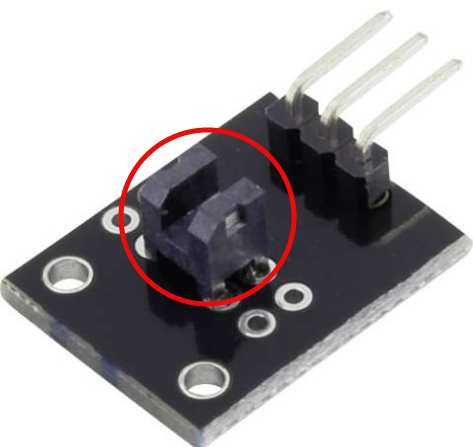
\includegraphics[width=0.5\textwidth, keepaspectratio]{./images/iduino_highlighted.png}
	\caption{The photoelectric sensor (Iduino 1485329) with the corresponding endpoints highlighted.}\label{img:iduino_highlighted}
\end{figure}	
We use this to simulate the entries of persons by passing a black stripe through each of the two sensors.
\subsection{Interrupt Handling}
We attach interrupt routines to both our sensors\footnote{as described here \url{https://www.arduino.cc/reference/de/language/functions/external-interrupts/attachinterrupt/}}. One advantage of this is, that the CPU can enter a power-save mode.\\
On our setup it was not possible to react to \textbf{RISING} (pin changes from low to high) and \textbf{LOW} (pin is low) simultaneously. Instead we chose to attach an interrupt to the \textbf{CHANGE} (pin changes from low to high or vice versa) and retrieve the state of the pin in the corresponding method for each pin. See \eqref{img:photo_model} for our setup.\\
\begin{figure}[p]
	\centering
	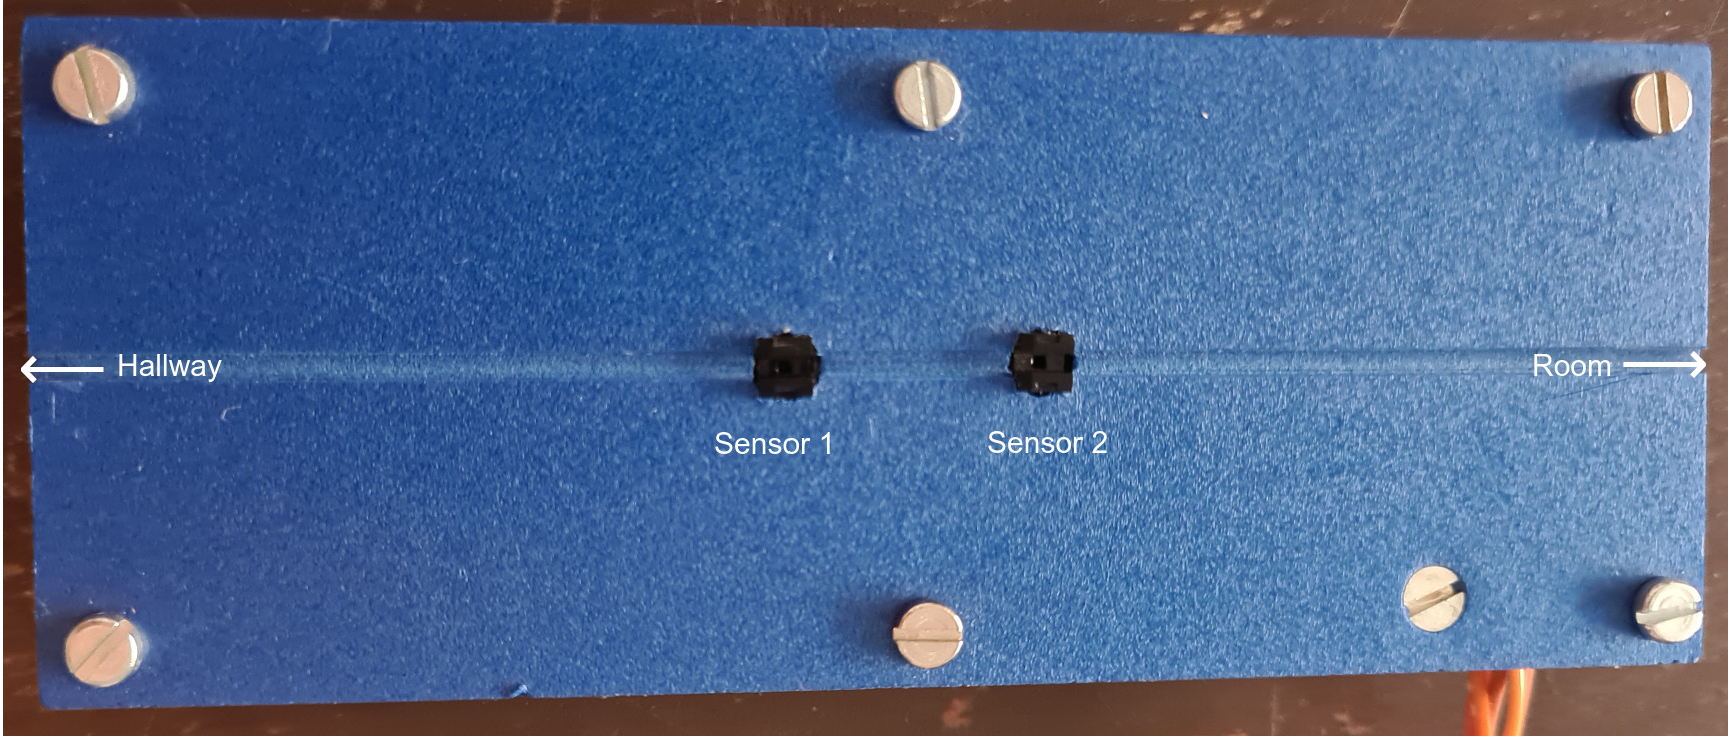
\includegraphics[width=\textwidth, keepaspectratio]{./images/photoelectric_model.png}
	\caption{Photoelectronic Sensors with our naming conventions and assumptions}\label{img:photo_model}
\end{figure}
It is important to add, that modeling a person, that would not activate both sensors (at least once) simultaneously is impossible. Assume for contradiction that a person only triggers one sensor at a time. Then it would be impossible to tell if they leave the sensor to the right or left. We therefore make the aforementioned assumption.\\
Theoretically, we could use some statistical modeling using time as a third variable but this would be outside the scope of this exercise.
Therefore we are left with the following states:
\begin{table}[H]
	\centering
\begin{tabularx}{.9\textwidth}{| l | X |}
			\hline
			Event & State Progression \\
			\hline
			Entering & $\mathit{isHigh1} \wedge \neg \mathit{isHigh2} \Longrightarrow \mathit{isHigh1} \wedge \mathit{isHigh2} \Longrightarrow \neg \mathit{isHigh1} \wedge \mathit{isHigh2} \Longrightarrow \neg \mathit{isHigh1} \wedge \neg \mathit{isHigh2}$\\
			\hline
			Peeking (Outside) & $\mathit{isHigh1} \wedge \neg \mathit{isHigh2} \Longrightarrow \mathit{isHigh1} \wedge \mathit{isHigh2} \Longrightarrow \mathit{isHigh1} \wedge \neg \mathit{isHigh2} \Longrightarrow \neg \mathit{isHigh1} \wedge \neg \mathit{isHigh2}$\\
			\hline
			Peeking (Outside short) & $\mathit{isHigh1} \wedge \neg \mathit{isHigh2} \Longrightarrow \neg \mathit{isHigh1} \wedge \neg \mathit{isHigh2}$\\
			\hline
			Exiting &  $\neg \mathit{isHigh1} \wedge \mathit{isHigh2} \Longrightarrow \mathit{isHigh1} \wedge \mathit{isHigh2} \Longrightarrow \mathit{isHigh1} \wedge \neg \mathit{isHigh2} \Longrightarrow \neg \mathit{isHigh1} \wedge \neg \mathit{isHigh2}$\\
			\hline
			Peeking (Inside) & $\neg \mathit{isHigh1} \wedge \mathit{isHigh2} \Longrightarrow \mathit{isHigh1} \wedge \mathit{isHigh2} \Longrightarrow \neg \mathit{isHigh1} \wedge \mathit{isHigh2} \Longrightarrow \neg \mathit{isHigh1} \wedge \neg \mathit{isHigh2}$\\
			\hline
			Peeking (Inside short) & $\neg \mathit{isHigh1} \wedge \mathit{isHigh2} \Longrightarrow \neg \mathit{isHigh1} \wedge \neg \mathit{isHigh2}$\\
			\hline
		\end{tabularx}
		\caption{Possible states for our model. "$\Longrightarrow$" indicates a change in the (sensor-) state. \textit{isHigh1} and \textit{isHigh2} are boolean variables, that indicate if sensor 1 or sensor 2 respectively is high.}
		\label{tab:possible_states}
\end{table}
Without loss of generality we assume $\neg \mathit{isHigh1} \and \neg \mathit{isHigh2}$, namely both sensors having a \textbf{LOW} reading, as our initial state and left it out in the table for readability.\\
Every other chain of events is not relevant for our use case, namely keeping track of the current amount of people in a room. The cases 1 - 3 (People coming from the hallway trying to "enter") and 4 - 6 (People coming from the room trying to "exit") are symmetric and were written out for completeness sake.\\
\newpage
% Sources
\printbibliography

\end{sloppypar}

\end{document}
